
\documentclass[11pt]{article}

% general packages without options
\usepackage{amsmath,amssymb,bbm}
% graphics
\usepackage{graphicx}
% text formatting
\usepackage[document]{ragged2e}
\usepackage{pagecolor,color}

\newcommand{\noun}[1]{\textsc{#1}}

\usepackage[utf8]{inputenc}
\usepackage[T1]{fontenc}
% geometry
\usepackage[margin=2cm]{geometry}

\usepackage{multicol}
\usepackage{setspace}

\usepackage{natbib}
\setlength{\bibsep}{0.0pt}

%\usepackage[french]{babel}

% layout : use fancyhdr package
%\usepackage{fancyhdr}
%\pagestyle{fancy}

% variable to include comments or not in the compilation ; set to 1 to include
\def \draft {1}


% writing utilities

% comments and responses
%  -> use this comment to ask questions on what other wrote/answer questions with optional arguments (up to 4 answers)
\usepackage{xparse}
\usepackage{ifthen}
\DeclareDocumentCommand{\comment}{m o o o o}
{\ifthenelse{\draft=1}{
    \textcolor{red}{\textbf{C : }#1}
    \IfValueT{#2}{\textcolor{blue}{\textbf{A1 : }#2}}
    \IfValueT{#3}{\textcolor{ForestGreen}{\textbf{A2 : }#3}}
    \IfValueT{#4}{\textcolor{red!50!blue}{\textbf{A3 : }#4}}
    \IfValueT{#5}{\textcolor{Aquamarine}{\textbf{A4 : }#5}}
 }{}
}

% todo
\newcommand{\todo}[1]{
\ifthenelse{\draft=1}{\textcolor{red!50!blue}{\textbf{TODO : \textit{#1}}}}{}
}


\usepackage[colorlinks=true]{hyperref}

\usepackage{ulem}


\makeatletter


\makeatother


\begin{document}


%%%%
% Diffusion :
%  X Geotamtam
%  X quanti 
%  X discuss iscpif
%  X ovenstreet
%  X lvmt
% 



\title{
\textit{ECTQG 2019}\medskip\\
New methods and Tools in the Exploration of Geosimulation Models\medskip\\
\textit{Special session proposal}
}

\date{}

\maketitle

\justify

\pagenumbering{gobble}


% the name(s) of the organiser(s)
% a short title for the session
% a half-page description of its scope
% intentions and plans to publish a special issue in a journal

% -> send to 2019@ectqg.eu

\section*{Organizers}

J. Raimbault and R. Reuillon (UPS CNRS 3611 ISC-PIF)


\section*{Scope}

The study of geosimulation models has always been associated to advanced sensitivity analysis, calibration and model exploration methods. The complexity of space makes these tools even more crucial than for aspatial simulation models, and furthermore requires specific methods to be designed. Typical issues in that context are illustrated by the different components of the OpenMOLE software, which is a platform specifically developed for model exploration and high performance computing. This platform allows to (i) embed any model as a black box in experiment workflows; (ii) use state-of-the-art calibration algorithms and sensitivity analysis methods; (iii) transparently access high performance computing environments. New components are specifically being developed for spatial models, including for example the generation of synthetic urban configurations or the assessment of the effect of spatial noise in input data. Following this approach, the aim of this session is to explore new trends in such methods and tools in the specific case of geosimulation models. Contributions can be related to the following questions: (i) methodological contributions including new methods and tools related to the study of geosimulation models (ii) issues specific to geosimulation models in developing model exploration methods, for example how taking into account space modifies existing methods, or how to deal with the higher complexity of spatial models; (iii) case studies of geosimulation models in which intensive computation and model exploration methods plays a crucial role. The convergence of diverse points of view, including for example methodological, theoretical, and thematical contributions, shall be an avenue to open new contributions and foster new perspectives in that field.


\section*{Special issue}

We are considering to propose a special issue for the contributions either in Environment and Planning B, or in Computer, Environment and Urban Systems.
% CEUS ?
% EPB ?


%\vspace{1cm}

\centering

\includegraphics[width=0.3\linewidth]{openmole}\hspace{0.5cm}
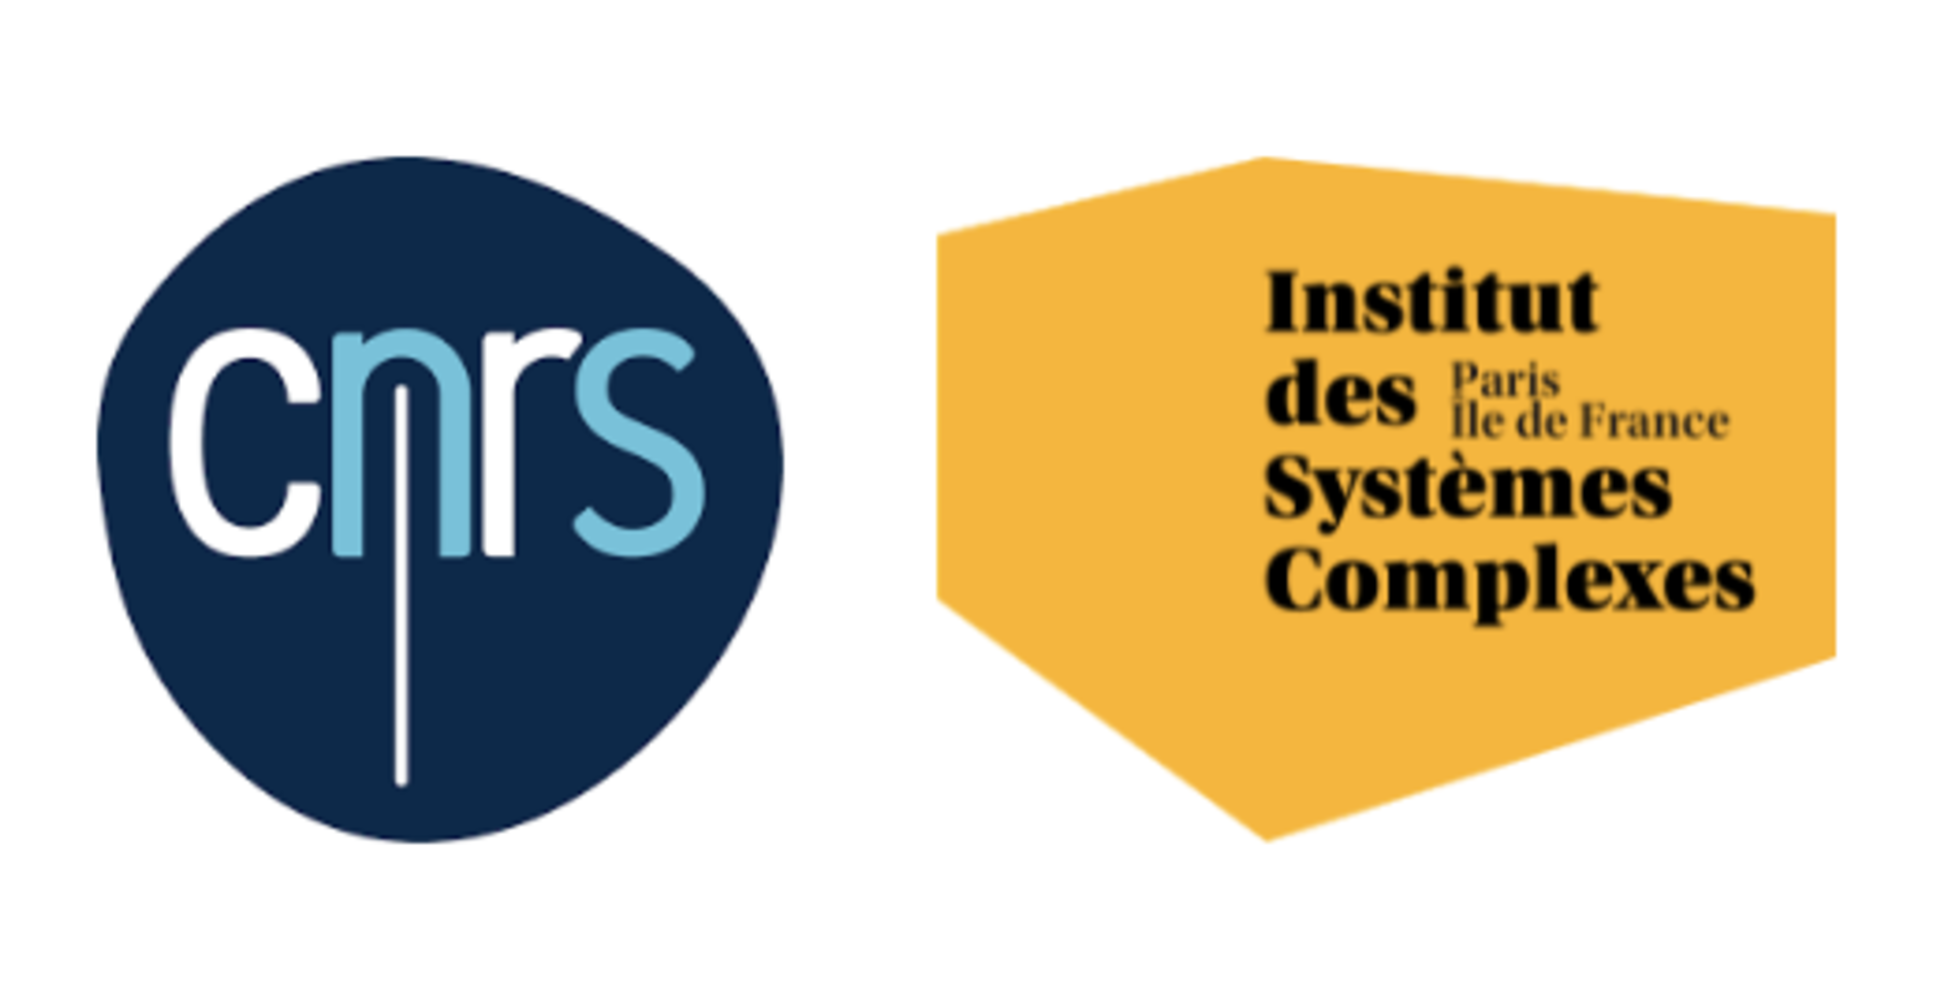
\includegraphics[width=0.3\linewidth]{isc}


%The study of complexity can not be anymore dissociated from intensive computational practices. Modeling and simulation have indeed taken a crucial role in the extraction of knowledge, especially in the study of systems with a high complexity such as socio-technical systems. Quantitative geography is a perfect illustration of how methodological, technical, empirical and theoretical advances necessarily strongly bind together: the use of computation centers in the seventies would be comparable to the current democratization of grid computing which impact dramatically changes the way social science is practiced. 
%This trend is propeled by the development of dedicated tools such as the \href{http://openmole.org/}{OpenMOLE software} for model exploration, guiding a progressive shift in simulation practices. Three fundamental innovative axis distinguish this new philosophy and technology compared to existing approaches in simulation: (i) the embedding of models within workflows, making model coupling and multi-modeling easier; (ii) the provision of novel heuristic methods for model exploration; and (iii) the transparent access to various intensive computation infrastructures. This approach can be seen as a knowledge accelerator which favors the construction of a robust and experimental social science, by the introduction of tools to deal with main requirements for it: multiple heterogenous models can be compared and coupled in an interdisciplinary approach within a new incremental methodology, models and workflows are open to ensure reproducibility, the behavior of models is better known with specific methods for model optimization, calibration and exploration. 
%The aim of this symposium is take a reflexive positioning on these trends, situate them regarding similar practices, and establish the most crucial future issues to be tackled within that stream of research.




%\section*{Invited speakers}
%\begin{itemize}
%    \item \textbf{Pr. Denise Pumain}, UMR CNRS 8504 Géographie-cités, Université Paris 1 - PI of the ERC advanced grant project Geodivercity.
%   \item \textbf{Dr. Romain Reuillon}, UPS CNRS 3611 ISC-PIF - Lead of the OpenMole project.
%    \item \textbf{Pr. Franck Varenne}, Université de Rouen.
%    \item \textbf{Pr. Celine Rozenblat}, Université de Lausanne.
%    \item \textbf{Simon Carignon}, Barcelona Supercomputing Center.
%\end{itemize}

%\section*{Organizers}
%\begin{itemize}
%	\item Juste Raimbault, ISC-PIF, \href{mailto:juste.raimbault@iscpif.fr}{juste.raimbault@iscpif.fr}
%	\item Romain Reuillon, ISC-PIF, \href{mailto:romain.reuillon@iscpif.fr}{romain.reuillon@iscpif.fr}
%\end{itemize}




%%%%%%%%%%%%%%%%%%%%
%% Biblio
%%%%%%%%%%%%%%%%%%%%
%\tiny

%\begin{multicols}{2}

%\setstretch{0.3}
%\setlength{\parskip}{-0.4em}


%\bibliographystyle{apalike}
%\bibliography{biblio}
%\end{multicols}



\end{document}
